% chktex-file 29
% chktex-file 13
\documentclass{report}
\usepackage{setspace}
\usepackage[a4paper, total={7in, 9in}]{geometry}
\usepackage[fleqn]{amsmath}
\usepackage{empheq}
\usepackage{amssymb}
\usepackage{amsthm}
\usepackage{gensymb}
\usepackage[fleqn]{cases}
\usepackage{multicol}
\usepackage{color}
\usepackage{stix}
\usepackage{chngcntr}
\usepackage{tikz}
\usepackage{enumitem}
\usetikzlibrary{calc,matrix}

\counterwithout{equation}{chapter}
\setlength{\columnseprule}{1pt}
\setlength{\columnsep}{24pt}
\setcounter{chapter}{11}
\hfuzz=100pt

\newtheorem{theorem}{Theorem}

\begin{document}
\newcommand{\sol}[1]{

    \noindent \textbf{Sol.}
}
\newcommand{\prooff}[1]{

    \noindent \textbf{Proof.}
}
\newcommand\m[1]{\begin{pmatrix}#1\end{pmatrix}}
\newcommand\vm[1]{\begin{vmatrix}#1\end{vmatrix}}
\newenvironment{amatrix}[1]{%
    \left(\begin{array}{@{}*{#1}{c}|c@{}}
        }{%
    \end{array}\right)
}
\begin{titlepage}
    \raggedleft{}
    \rule{1pt}{\textheight}
    \hspace{0.02\textwidth}
    \parbox[b]{0.75\textwidth}{

    {\Huge\bfseries Solution Book of \\[0.5\baselineskip] Mathematic}\\[2\baselineskip]
    {\large\textit{Ssnior 2 Part I}}\\[4\baselineskip]
    {\Large\textsc{MELVIN CHIA}}

    \vspace{0.5\textheight}

    {\noindent Written on 9 October 2022}\\[\baselineskip]
    }

\end{titlepage}

\doublespacing{}
\tableofcontents
\singlespacing{}
\newpage

\begin{multicols}{2}
    \section{Revision Exercise 14}

    Calculate the following (Question 1 to 4):

    \begin{enumerate}[wide, labelwidth=!, labelindent=0pt]

        \item $5\m{
                      -3 & -1 \\
                      3  & 4
                  } + 4\m{
                      6 & 2  \\
                      1 & -1
                  }$
              \sol{}
              \begin{flalign*}
                      & 5\m{
                  -3  & -1    \\
                  3   & 4
                  } + 4\m{
                  6   & 2     \\
                  1   & -1
                  }           \\
                      & = \m{
                  -15 & -5    \\
                  15  & 20
                  } + \m{
                  24  & 8     \\
                  4   & -4
                  }           \\
                      & = \m{
                  9   & 3     \\
                  19  & 16
                  }
              \end{flalign*}

        \item $-4\m{
                      3  & 0 \\
                      -1 & 5
                  } - 3\m{
                      1  & 0 \\
                      -1 & -1
                  }$
              \sol{}
              \begin{flalign*}
                      & -4\m{
                  3   & 0     \\
                  -1  & 5
                  } - 3\m{
                  1   & 0     \\
                  -1  & -1
                  }           \\
                      & = \m{
                  -12 & 0     \\
                  4   & -20
                  } - \m{
                  3   & 0     \\
                  -3  & -3
                  }           \\
                      & = \m{
                  -15 & 0     \\
                  7   & 17
                  }
              \end{flalign*}

        \item $\m{
                      2 & 6  & -1 \\
                      8 & -4 & 3  \\
                      5 & 7  & -2 \\
                  } + \m{
                      4  & -2 & 1 \\
                      -2 & 1  & 0 \\
                      -3 & 5  & -4
                  }$
              \sol{}
              \begin{flalign*}
                     & \m{
                  2  & 6     & -1 \\
                  8  & -4    & 3  \\
                  5  & 7     & -2
                  } + \m{
                  4  & -2    & 1  \\
                  -2 & 1     & 0  \\
                  -3 & 5     & -4
                  }               \\
                     & = \m{
                  6  & 4     & 0  \\
                  6  & -3    & 3  \\
                  2  & 12    & -6
                  }
              \end{flalign*}

        \item $2\m{
                      1 & -3 & 5  \\
                      7 & 2  & 0  \\
                      2 & 4  & -4
                  } - \m{
                      -2 & -6 & 2  \\
                      -5 & 1  & 1  \\
                      0  & 0  & -2
                  }$
              \sol{}
              \begin{flalign*}
                     & 2\m{
                  1  & -3    & 5  \\
                  7  & 2     & 0  \\
                  2  & 4     & -4
                  } - \m{
                  -2 & -6    & 2  \\
                  -5 & 1     & 1  \\
                  0  & 0     & -2
                  }               \\
                     & = \m{
                  2  & -6    & 10 \\
                  14 & 4     & 0  \\
                  4  & 8     & -8
                  } - \m{
                  -2 & -6    & 2  \\
                  -5 & 1     & 1  \\
                  0  & 0     & -2
                  }               \\
                     & = \m{
                  4  & 0     & 8  \\
                  19 & 3     & -1 \\
                  4  & 8     & -6
                  }
              \end{flalign*}

    \end{enumerate}

    \begin{enumerate}[wide, labelwidth=!, labelindent=0pt]
        \setcounter{enumi}{4}

        \item Given that $\m{2\\-3} + 3\m{5 \\ y} = \m{x\\y}$, find the value of $x$ and $y$.
              \sol{}
              \begin{flalign*}
                  \m{2                                    \\-3} + 3\m{5 \\ y} &= \m{x\\y} \\
                  \m{2                                    \\-3} + \m{15 \\ 3y} &= \m{x\\y} \\
                  \m{17                                   \\ -3 + 3y} &= \m{x\\y} \\
                  x             & = 17                    \\
                  y             & = -3 + 3y               \\
                  2y            & = 3                     \\
                  y             & = \frac{3}{2}           \\
                  \therefore\ x & = 17, \ y = \frac{3}{2}
              \end{flalign*}

        \item Let $P = \m{ 3 & -2 & 1 \\ -1 & 2 &-3 \\ 4 & 0 & -2 }$, $Q = \m{ 1 & -5 & -4 \\
                      -2 & 0 & 6 \\ 3 & 2 & 3 }$ and $R = \m{ 4 & 0 & 5 \\ 1 & -2 & -7 \\ 0 & -2 & 1
                  }$. Find the following:

              \begin{enumerate}

                  \item $2Q + R'$
                        \sol{}
                        \begin{flalign*}
                            2Q + R' & = 2\m{ 1 & -5 & -4 \\
                            -2      & 0        & 6       \\ 3 & 2 & 3 } + \m{
                            4       & 0        & 5       \\
                            1       & -2       & -7      \\
                            0       & -2       & 1
                            }'                           \\
                                    & = \m{
                            2       & -10      & -8      \\
                            -4      & 0        & 12      \\
                            6       & 4        & 6
                            } + \m{
                            4       & 1        & 0       \\
                            0       & -2       & -2      \\
                            5       & -7       & 1
                            }                            \\
                                    & = \m{
                            6       & -9       & -8      \\
                            -4      & -2       & 10      \\
                            11      & -3       & 7
                            }
                        \end{flalign*}

                  \item $(P-R) + 2Q'$
                        \sol{}
                        \begin{flalign*}
                                & (P-R) + 2Q'                \\
                                & = \m{ 3          & -2 & 1  \\ -1 & 2 & -3 \\ 4 & 0 & -2 } - \m{
                            4   & 0                & 5       \\
                            1   & -2               & -7      \\
                            0   & -2               & 1
                            }                                \\
                                & \ \ \ \ + 2\m{ 1 & -5 & -4 \\
                            -2  & 0                & 6       \\ 3 & 2 & 3 }'                          &\\
                                & = \m{
                            -1  & -2               & -4      \\
                            -2  & 4                & 4       \\
                            4   & 2                & -3
                            } + \m{
                            2   & -4               & 6       \\
                            -10 & 0                & 4       \\
                            -8  & 12               & 6
                            }                                \\
                                & = \m{
                            1   & 6                & 2       \\
                            -12 & 4                & 8       \\
                            -4  & 14               & 3
                            }
                        \end{flalign*}

                  \item $[2(Q-P)]'$
                        \sol{}
                        \begin{flalign*}
                                              & [2(Q-P)]'             &                \\
                                              & = \left\{2\left[\m{ 1 & -5        & -4 \\
                            -2                & 0                     & 6              \\
                            3                 & 2                     & 3 } - \m{
                            3                 & -2                    & 1              \\
                            -1                & 2                     & -3             \\
                            4                 & 0                     & -2
                            }\right]\right\}' &                                        \\
                                              & = \left[2\m{
                            -2                & -3                    & -5             \\
                            -1                & -2                    & 9              \\
                            -1                & 2                     & 5
                            }\right]'         &                                        \\
                                              & = \m{
                            -4                & -6                    & -10            \\
                            -2                & -4                    & 18             \\
                            -2                & 4                     & 10
                            }'                &                                        \\
                                              & = \m{
                            -4                & -2                    & -2             \\
                            -6                & -4                    & 4              \\
                            -10               & 18                    & 10
                            }
                        \end{flalign*}

                  \item $(R'-Q)'$
                        \sol{}
                        \begin{flalign*}
                            (R'-Q)' & = \left[\m{
                            4       & 0           & 5  \\
                            1       & -2          & -7 \\
                            0       & -2          & 1
                            }' - \m{
                            1       & -5          & -4 \\
                            -2      & 0           & 6  \\
                            3       & 2           & 3
                            }\right]'                  \\
                                    & = \m{
                            4       & 0           & 5  \\
                            1       & -2          & -7 \\
                            0       & -2          & 1
                            } - \m{
                            1       & -5          & -4 \\
                            -2      & 0           & 6  \\
                            3       & 2           & 3
                            }'                         \\
                                    & = \m{
                            4       & 0           & 5  \\
                            1       & -2          & -7 \\
                            0       & -2          & 1
                            } - \m{
                            1       & -2          & 3  \\
                            -5      & 0           & 2  \\
                            -4      & 6           & 3
                            }                          \\
                                    & = \m {
                            3       & 2           & 2  \\
                            6       & -2          & -9 \\
                            4       & -8          & -2
                            }
                        \end{flalign*}

              \end{enumerate}

        \item Let $M = \m{ -1 & 0 \\ 4 & -3 \\ 2 & 4 }$ and $N = \m{ 3 & 6 \\ 7 & -1 \\ -4 &
                      2 }$. Find the matrix $X$ in the following equations:

              \begin{enumerate}

                  \item $2N - 3M = 2M - X$
                        \sol{}
                        \begin{flalign*}
                            2N - 3M & = 2M - X  \\
                            X       & = 5M - 2N \\
                                    & = 5\m{
                            -1      & 0         \\
                            4       & -3        \\
                            2       & 4
                            } - 2\m{
                            3       & 6         \\
                            7       & -1        \\
                            -4      & 2
                            }                   \\
                                    & = \m{
                            -5      & 0         \\
                            20      & -15       \\
                            10      & 20
                            } - \m{
                            6       & 12        \\
                            14      & -2        \\
                            -8      & 4
                            }                   \\
                                    & = \m{
                            -11     & -12       \\
                            6       & -13       \\
                            18      & 16
                            }
                        \end{flalign*}

                  \item $2(M-2N) + X = M + N$
                        \sol{}
                        \begin{flalign*}
                            2(M-2N) + X & = M + N           \\
                            X           & = M + N - 2(M-2N) \\
                                        & = M + N - 2M + 4N \\
                                        & = -M + 5N         \\
                                        & = -\m{
                            -1          & 0                 \\
                            4           & -3                \\
                            2           & 4
                            } + 5\m{
                            3           & 6                 \\
                            7           & -1                \\
                            -4          & 2
                            }                               \\
                                        & = \m{
                            1           & 0                 \\
                            -4          & 3                 \\
                            -2          & -4
                            } + \m{
                            15          & 30                \\
                            35          & -5                \\
                            -20         & 10
                            }                               \\
                                        & = \m{
                            16          & 30                \\
                            31          & -2                \\
                            -22         & 6
                            }
                        \end{flalign*}

                  \item $(M + 2N)' = X$
                        \sol{}
                        \begin{flalign*}
                            (M + 2N)' & = X              \\
                            X         & = (M + 2N)'      \\
                                      & = \left[\m{
                            -1        & 0                \\
                            4         & -3               \\
                            2         & 4
                            } + 2\m{
                            3         & 6                \\
                            7         & -1               \\
                            -4        & 2
                            }\right]'                    \\
                                      & = \left[\m{
                            -1        & 0                \\
                            4         & -3               \\
                            2         & 4
                            } + \m{
                            6         & 12               \\
                            14        & -2               \\
                            -8        & 4
                            }      \right]               \\
                                      & = \m{
                            5         & 12               \\
                            18        & -5               \\
                            -6        & 8
                            }'                           \\
                                      & = \m{
                            5         & 18          & -6 \\
                            12        & -5          & 8
                            }
                        \end{flalign*}

                  \item $3N' - M' = 2X$
                        \sol{}
                        \begin{flalign*}
                            3N' - M' & = 2X               \\
                            2X       & = (3N - M)'        \\
                                     & = \left[3\m{
                            3        & 6                  \\
                            7        & -1                 \\
                            -4       & 2
                            } - \m{
                            -1       & 0                  \\
                            4        & -3                 \\
                            2        & 4
                            }\right]'                     \\
                                     & = \left[\m{
                            9        & 18                 \\
                            21       & -3                 \\
                            -12      & 6
                            } - \m{
                            -1       & 0                  \\
                            4        & -3                 \\
                            2        & 4
                            }\right]'                     \\
                                     & = \m{
                            10       & 18                 \\
                            17       & 0                  \\
                            -14      & 2
                            }'                            \\
                                     & = \m{
                            10       & 17           & -14 \\
                            18       & 0            & 2
                            }                             \\
                            X        & = \m{
                            5        & \frac{17}{2} & -7  \\
                            9        & 0            & 1
                            }
                        \end{flalign*}

              \end{enumerate}

    \end{enumerate}

    \noindent Of the following matrices, determine if $AB$ and $BA$ are defined. If any of them is
    defined, find the value of them (Question 8 to 11):

    \begin{enumerate}[wide, labelwidth=!, labelindent=0pt]
        \setcounter{enumi}{7}

        \item $A = \m{
                      3 \\
                      1 \\
                      4
                  }$, $B = \m{
                      1  & 0 & 2  \\
                      -2 & 0 & 1  \\
                      1  & 1 & -1
                  }$
              \sol{}
              \begin{flalign*}
                     & \because\ \parbox{2.5in}{The number of columns of $A$ is not equal to the number of rows of
                  $B$}                                                                                                 \\ & \therefore\ \text{$AB$ is not defined} \\\\  & \because\ \parbox{2.5in}{The number of columns of $B$ is equal to the number of rows of $A$}
                  \\ & \therefore\ \text{$BA$ is defined} \\ & \therefore\ BA = \m{ 1 & 0 & 2 \\
                  -2 & 0                                                                                           & 1 \\ 1 & 1 & -1 } \m{ 3 \\ 1 \\ 4 } = \m{ 11 \\ -2 \\ 0 }
              \end{flalign*}

        \item $A = \m{
                      -5 & 4 & 3 \\
                      1  & 2 & 3
                  }$, $B = \m{
                      -2 & 1  \\
                      -3 & 0  \\
                      1  & -4
                  }$
              \sol{}
              \begin{flalign*}
                      & \because\ \parbox{2.5in}{The number of columns of $A$ is equal to the number of rows of $B$}
                  \\ & \therefore\ \text{$AB$ is defined} \\ & \therefore\ AB = \m{ -5 & 4 & 3 \\
                  1   & 2                                                                                            & 3 } \m{ -2 & 1 \\ -3 & 0 \\ 1 & -4 } = \m{ 1 & -17 \\ -5 & -11 } \\\\  &
                    \because\ \parbox{2.5in}{The number of columns of $B$ is equal to the number of rows of $A$}
                  \\ & \therefore\ \text{$BA$ is defined} \\ & \therefore\ BA = \m{ -2 & 1 \\ -3
                      & 0                                                                                                             \\ 1 & -4 } \m{ -5 & 4 & 3 \\ 1 & 2 & 3 } \\ &= \m{ 11 & -6 & -3 \\ 13  &
                  -12 & -9                                                                                                            \\ -9 & -4 & -9 }
              \end{flalign*}

        \item $A = \m{
                      3  & 2 & -1 \\
                      5  & 4 & 0  \\
                      -2 & 6 & 1
                  }$, $B = \m{
                      9  & 0 \\
                      -7 & 1 \\
                      2  & 3
                  }$
              \sol{}
              \begin{flalign*}
                    & \because\ \parbox{2.5in}{The number of columns of $A$ is equal to the number of rows of $B$}
                  \\ & \therefore\ \text{$AB$ is defined} \\ & \therefore\ AB = \m{ 3 & 2 & -1 \\
                  5 & 4                                                                                            & 0 \\ -2 & 6 & 1 } \m{ 9 & 0 \\ -7 & 1 \\ 2 & 3 } = \m{ 11 & -1 \\ 17 &
                  4                                                                                                    \\ -58 & 9 } \\\\  & \because\ \parbox{2.5in}{The number of columns of $B$ is not equal to the number of rows of
                  $A$}                                                                                                 \\ & \therefore\ \text{$BA$ is not defined}
              \end{flalign*}

        \item $A = \m{
                      2 & 0 \\
                      4 & 1
                  }$, $B = \m{
                      3 & 0 \\
                      1 & 4 \\
                      5 & 2
                  }$
              \sol{}
              \begin{flalign*}
                   & \because\ \parbox{2.5in}{The number of columns of $A$ is not equal to the number of rows of
                  $B$}                                                                                           \\ & \therefore\ \text{$AB$ is not defined} \\\\  & \because\ \parbox{2.5in}{The number of columns of $B$ is equal to the number of rows of $A$}
                  \\ & \therefore\ \text{$BA$ is defined} \\ & \therefore\ BA = \m{ 3 & 0 \\ 1 &
                  4                                                                                              \\ 5 & 2 } \m{ 2 & 0 \\ 4 & 1 } = \m{ 6 & 0 \\ 10 & 4 \\ 18 & 2 }
              \end{flalign*}

    \end{enumerate}

    \begin{enumerate}[wide, labelwidth=!, labelindent=0pt]
        \setcounter{enumi}{11}

        \item Given that $A = \m{ a & 3a \\ 2b & b }$, $B = \m{ 3\\ 2 }$, $AB = \m{ 45 \\ 48
                  }$, find the value of $a$ and $b$. \sol{}
              \begin{flalign*}
                  AB = \m{ a & 3a       \\ 2b & b } \m{ 3 \\ 2 } &= \m{ 45 \\ 48 }\\
                  \m{
                  3a + 6a               \\
                  6b + 2b
                  }          & = \m{ 45 \\ 48 }\\
                  9a         & = 45     \\
                  8b         & = 48     \\
                  a          & = 5      \\
                  b          & = 6
              \end{flalign*}

        \item Given that $A = \m{ 3 & 0 \\ 0 & 4 }$, $B = \m{ a & b \\ 0 & c }$, $A + B =
                  AB$, find the value of $a$, $b$ and $c$. \sol{}
              \begin{flalign*}
                  A + B                        & = AB                  \\
                  \m{ 3                        & 0                     \\ 0 & 4 } + \m{ a & b \\ 0 & c } &= \m{ 3 & 0 \\ 0 & 4 } \m{ a & b \\ 0 & c } \\
                  \m{ 3 + a                    & b                     \\ 0 & 4 + c } &= \m{ 3a & 3b \\ 0 & 4c } \\
                  3 + a                        & = 3a                  \\
                  2a                           & = 3                   \\
                  b                            & = 3b                  \\
                  2b                           & = 0                   \\
                  4 + c                        & = 4c                  \\
                  3c                           & = 4                   \\
                  a          = \frac{3}{2},\ b & = 0,\ c = \frac{4}{3}
              \end{flalign*}

    \end{enumerate}

    \noindent Find the value of the following determinants (Question 14 to 22):

    \begin{enumerate}[wide, labelwidth=!, labelindent=0pt]
        \setcounter{enumi}{13}

        \item $\vm{
                      20 & 15\\
                      8 & 6
                  }$
              \sol{}
              \begin{flalign*}
                  \vm{
                  20 & 15                        \\
                  8  & 6
                  }  & = 20 \cdot 6 - 15 \cdot 8 \\
                     & = 120 - 120               \\
                     & = 0
              \end{flalign*}

        \item $\vm{
                      6 & -7\\
                      15 & -2
                  }$
              \sol{}
              \begin{flalign*}
                  \vm{
                  6  & -7                           \\
                  15 & -2
                  }  & = 6 \cdot -2 - (-7) \cdot 15 \\
                     & = -12 + 105                  \\
                     & = 93
              \end{flalign*}

        \item $\vm{
                      -4 & -10\\
                      12 & 7
                  }$
              \sol{}
              \begin{flalign*}
                  \vm{
                  -4 & -10                           \\
                  12 & 7
                  }  & = -4 \cdot 7 - (-10) \cdot 12 \\
                     & = -28 + 120                   \\
                     & = 92
              \end{flalign*}

        \item $\vm{
                      3 & 3 & -6\\
                      2 & -2 & 0\\
                      3 & 0 & -3
                  }$
              \begin{center}
                  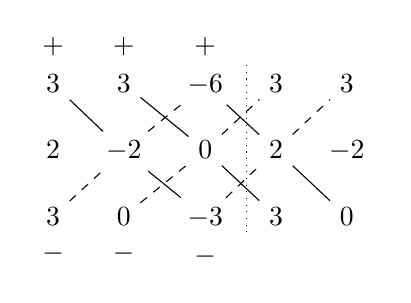
\begin{tikzpicture}
                      \matrix [%
                          matrix of math nodes,
                          column sep=1em,
                          row sep=1em
                      ] (sarrus) {%
                          3 & 3  & -6 & 3 & 3  \\
                          2 & -2 & 0  & 2 & -2 \\
                          3 & 0  & -3 & 3 & 0  \\
                      };

                      \path ($(sarrus-1-3.north east)+(0.5em,0)$) edge[dotted] ($(sarrus-3-3.south east)+(0.5em,0)$)
                      (sarrus-1-1)                          edge         (sarrus-2-2)
                      (sarrus-2-2)                          edge         (sarrus-3-3)
                      (sarrus-1-2)                          edge         (sarrus-2-3)
                      (sarrus-2-3)                          edge         (sarrus-3-4)
                      (sarrus-1-3)                          edge         (sarrus-2-4)
                      (sarrus-2-4)                          edge         (sarrus-3-5)
                      (sarrus-3-1)                          edge[dashed] (sarrus-2-2)
                      (sarrus-2-2)                          edge[dashed] (sarrus-1-3)
                      (sarrus-3-2)                          edge[dashed] (sarrus-2-3)
                      (sarrus-2-3)                          edge[dashed] (sarrus-1-4)
                      (sarrus-3-3)                          edge[dashed] (sarrus-2-4)
                      (sarrus-2-4)                          edge[dashed] (sarrus-1-5);

                      \foreach \c in {1,2,3} {\node[anchor=south] at (sarrus-1-\c.north) {$+$};};
                      \foreach \c in {1,2,3} {\node[anchor=north] at (sarrus-3-\c.south) {$-$};};
                  \end{tikzpicture}
              \end{center}
              \sol{}
              \begin{flalign*}
                  \vm{
                  3 & 3                          & -6 \\
                  2 & -2                         & 0  \\
                  3 & 0                          & -3
                  } & = 18 + 0 + 0 - 36 - 0 + 18      \\
                    & = 0
              \end{flalign*}

        \item $\vm{
                      5 & 7 & 1\\
                      -3 & 6 & 9\\
                      4 & 7 & 3
                  }$
              \begin{center}
                  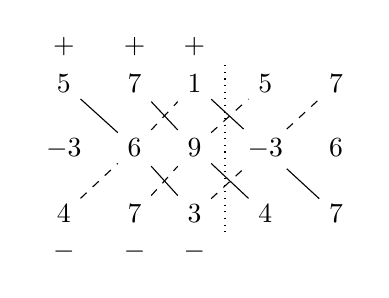
\begin{tikzpicture}
                      \matrix [%
                          matrix of math nodes,
                          column sep=1em,
                          row sep=1em
                      ] (sarrus) {%
                          5  & 7 & 1 & 5  & 7 \\
                          -3 & 6 & 9 & -3 & 6 \\
                          4  & 7 & 3 & 4  & 7 \\
                      };

                      \path ($(sarrus-1-3.north east)+(0.5em,0)$) edge[dotted] ($(sarrus-3-3.south east)+(0.5em,0)$)
                      (sarrus-1-1)                          edge         (sarrus-2-2)
                      (sarrus-2-2)                          edge         (sarrus-3-3)
                      (sarrus-1-2)                          edge         (sarrus-2-3)
                      (sarrus-2-3)                          edge         (sarrus-3-4)
                      (sarrus-1-3)                          edge         (sarrus-2-4)
                      (sarrus-2-4)                          edge         (sarrus-3-5)
                      (sarrus-3-1)                          edge[dashed] (sarrus-2-2)
                      (sarrus-2-2)                          edge[dashed] (sarrus-1-3)
                      (sarrus-3-2)                          edge[dashed] (sarrus-2-3)
                      (sarrus-2-3)                          edge[dashed] (sarrus-1-4)
                      (sarrus-3-3)                          edge[dashed] (sarrus-2-4)
                      (sarrus-2-4)                          edge[dashed] (sarrus-1-5);

                      \foreach \c in {1,2,3} {\node[anchor=south] at (sarrus-1-\c.north) {$+$};};
                      \foreach \c in {1,2,3} {\node[anchor=north] at (sarrus-3-\c.south) {$-$};};
                  \end{tikzpicture}
              \end{center}
              \sol{}
              \begin{flalign*}
                  \vm{
                  5  & 7                               & 1 \\
                  -3 & 6                               & 9 \\
                  4  & 7                               & 3
                  }  & = 90 + 252 - 21 - 24 - 315 + 63     \\
                     & = 45
              \end{flalign*}

        \item $\vm{
                      -2 & 7 & -4\\
                      3 & -5 & 2\\
                      -1 & 0 & -3
                  }$
              \begin{center}
                  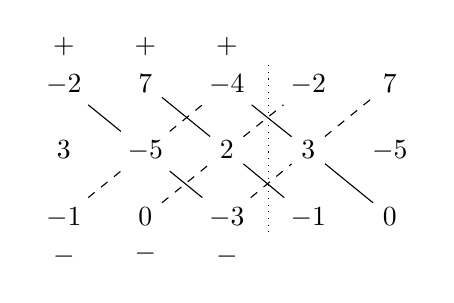
\begin{tikzpicture}
                      \matrix [%
                          matrix of math nodes,
                          column sep=1em,
                          row sep=1em
                      ] (sarrus) {%
                          -2 & 7  & -4 & -2 & 7  \\
                          3  & -5 & 2  & 3  & -5 \\
                          -1 & 0  & -3 & -1 & 0  \\
                      };

                      \path ($(sarrus-1-3.north east)+(0.5em,0)$) edge[dotted] ($(sarrus-3-3.south east)+(0.5em,0)$)
                      (sarrus-1-1)                          edge         (sarrus-2-2)
                      (sarrus-2-2)                          edge         (sarrus-3-3)
                      (sarrus-1-2)                          edge         (sarrus-2-3)
                      (sarrus-2-3)                          edge         (sarrus-3-4)
                      (sarrus-1-3)                          edge         (sarrus-2-4)
                      (sarrus-2-4)                          edge         (sarrus-3-5)
                      (sarrus-3-1)                          edge[dashed] (sarrus-2-2)
                      (sarrus-2-2)                          edge[dashed] (sarrus-1-3)
                      (sarrus-3-2)                          edge[dashed] (sarrus-2-3)
                      (sarrus-2-3)                          edge[dashed] (sarrus-1-4)
                      (sarrus-3-3)                          edge[dashed] (sarrus-2-4)
                      (sarrus-2-4)                          edge[dashed] (sarrus-1-5);

                      \foreach \c in {1,2,3} {\node[anchor=south] at (sarrus-1-\c.north) {$+$};};
                      \foreach \c in {1,2,3} {\node[anchor=north] at (sarrus-3-\c.south) {$-$};};
                  \end{tikzpicture}
              \end{center}
              \sol{}
              \begin{flalign*}
                  \vm{
                  -2 & 7                            & -4 \\
                  3  & -5                           & 2  \\
                  -1 & 0                            & -3
                  }  & = -30 - 14 - 0 + 20 + 0 + 63      \\
                     & = -39
              \end{flalign*}

        \item $\vm{
                      1 & 0 & -1\\
                      3 & -2 & 5\\
                      -1 & 1 & 3
                  }$
              \sol{}
              \begin{flalign*}
                  \vm{
                  1  & 0                   & -1 \\
                  3  & -2                  & 5  \\
                  -1 & 1                   & 3
                  }  & = \vm{
                  -2 & 5                        \\
                  1  & 3
                  } -3 \vm{
                  0  & -1                       \\
                  1  & 3
                  } - \vm{
                  0  & -1                       \\
                  -2 & 5
                  }                             \\
                     & = -11 - 3 + 2 = -12
              \end{flalign*}

        \item $\vm{
                      2 & 6 & 4\\
                      1 & 3 & 1\\
                      -2 & -6 & 5
                  }$
              \sol{}
              \begin{flalign*}
                  \vm{
                  2  & 6                                              & 4 \\
                  1  & 3                                              & 1 \\
                  -2 & -6                                             & 5
                  }  & = 3\vm{
                  2  & 2                                              & 4 \\
                  1  & 1                                              & 1 \\
                  -2 & -2                                             & 5
                  }  &                                                    \\
                     & = 0\ \ \ \ \ \text{(col 1 and 2 are the same)}     \\
              \end{flalign*}

        \item $\vm{
                      10 & 8 & -2\\
                      15 & 16 & -3\\
                      -5 & -4 & 1
                  }$
              \sol{}
              \begin{flalign*}
                  \vm{
                  10 & 8                                              & -2 \\
                  15 & 16                                             & -3 \\
                  -5 & -4                                             & 1
                  }  & = -5\vm{
                  2  & 8                                              & 2  \\
                  3  & 16                                             & 3  \\
                  -1 & -4                                             & -1
                  }                                                        \\
                     & = 0\ \ \ \ \ \text{(col 1 and 3 are the same)}
              \end{flalign*}

    \end{enumerate}

    \noindent Using the identities of determinant, prove the following equations (Question 23
    to 24):

    \begin{enumerate}[wide, labelwidth=!, labelindent=0pt]
        \setcounter{enumi}{22}

        \item $\vm{
                      bc & 1 & bc(b+c)\\
                      ca & 1 & ca(c+a)\\
                      ab & 1 & ab(a+b)
                  } = 0$

        \item $\vm{
                      a & 1 & a^2(b+c)\\
                      b & 1 & b^2(c+a)\\
                      c & 1 & c^2(a+b)
                  } = 0$

    \end{enumerate}

    Find the value of $x$ in the following expressions (Question 25 to 26):

    \begin{enumerate}[wide, labelwidth=!, labelindent=0pt]
        \setcounter{enumi}{24}

        \item $\vm{
                      2x & 3 & x+5\\
                      -3 & 2 & 1\\
                      2 & 1 & 0
                  } = 5x - 1$

        \item $\vm{
                      x+3 & 1 & 0\\
                      x & 3 & 0\\
                      1 & 0 & -x-2
                  } = x + 6$

    \end{enumerate}

    \begin{enumerate}[wide, labelwidth=!, labelindent=0pt]
        \setcounter{enumi}{26}

        \item Given an identity matrix $I = \m{ 1 & 0\\ 0 & 1 }$. Let $J = \m{ 0 & 1\\ -1 & 0
                  }$, ${(2I+J)}^{-1} = rI + sJ$, find the value of $r$ and $s$.

    \end{enumerate}

    \noindent Find the value of $a$ in the following matrices if they are non-inversible (Question 28 to 31):

    \begin{enumerate}[wide, labelwidth=!, labelindent=0pt]
        \setcounter{enumi}{27}

        \item $\m{
                      3 & a\\
                      -2 & 6
                  }$

        \item $\m{
                      5a + 2 & 4\\
                      6 & a
                  }$

        \item $\m{
                      -7 & a & 3\\
                      2 & -3 & 1\\
                      0 & -a & 4
                  }$

        \item $\m{
                      a & -1 & 0\\
                      4 & 0 & -2\\
                      a+4 & a & -8
                  }$

    \end{enumerate}

    \noindent Find the inverse of the following matrices (Question 32 to 37):

    \begin{enumerate}[wide, labelwidth=!, labelindent=0pt]
        \setcounter{enumi}{31}

        \item $\m{
                      2 & 5\\
                      2 & 3
                  }$

        \item $\m{
                      -2 & -1 \\
                      4 & 6
                  }$

        \item $\m{
                      1 & 0 & 3\\
                      3 & 1 & 9\\
                      -2 & 2 & -4
                  }$

        \item $\m{
                      1 & 2 & -3\\
                      2 & 1 & -2\\
                      -2 & 5 & 1
                  }$

        \item $\m{
                      4 & 1 & 0\\
                      0 & -2 & 3\\
                      0 & -4 & 4
                  }$

        \item $\m{
                      3 & 2 & 3\\
                      -1 & -3 & \\
                      1 & 0 & 3
                  }$

    \end{enumerate}

    \noindent Solve the following system of equations using the method of Gauss elimination (Question 38 to 41):

    \begin{enumerate}[wide, labelwidth=!, labelindent=0pt]
        \setcounter{enumi}{37}

        \item $\begin{cases}
                      2x - y + 4z = 5   \\
                      2x + 3y - 4z = -7 \\
                      x + y + z = 2
                  \end{cases}$

        \item $\begin{cases}
                      x - 2y - 3z = -4 \\
                      3x + y - 4z = -5 \\
                      2x + 4y - z = -5
                  \end{cases}$

        \item $\begin{cases}
                      x - 2y - z = 3  \\
                      4x - y + 2z = 1 \\
                      x + 3y = 5
                  \end{cases}$

        \item $\begin{cases}
                      2x - y - z = 0   \\
                      4x - 3y + 2z = 1 \\
                      3x - 2y - 4z = -1
                  \end{cases}$

    \end{enumerate}

    \noindent Solve the following system of equations using the Cramer's rule (Question 42 to 45):

    \begin{enumerate}[wide, labelwidth=!, labelindent=0pt]
        \setcounter{enumi}{41}

        \item $\begin{cases}
                      x - 3y - 2z = 1  \\
                      7x + 4y - 5z = 0 \\
                      3x + 9y + z = -1
                  \end{cases}$

        \item $\begin{cases}
                      x - 2y + 3z = 6   \\
                      2x + 3y - 4z = 20 \\
                      3x - 2y - 5z = 6
                  \end{cases}$

        \item $\begin{cases}
                      2x - 2x - 4z + 3 = 0 \\
                      2x + 3y + 4z - 2 = 0 \\
                      7x + 3y - 2z - 2 = 0
                  \end{cases}$

        \item $\begin{cases}
                      \frac{2}{x} - \frac{5}{y} + \frac{4}{z} = -3 \\
                      \frac{4}{x} + \frac{1}{y} - \frac{2}{z} = 7  \\
                      \frac{7}{x} - \frac{3}{z} = 4
                  \end{cases}$

    \end{enumerate}

\end{multicols}
\end{document}